Twitter affords us a large amount of publicly available data. The
following are the fields that we may extract for any given Twitter
user.

\begin{itemize}
\item \verb|created_at|: User account creation date
\item \verb|description|: User account description
\item \verb|favorites_count|: How many Tweets has the User favorited.
\item \verb|followers_count|: How many followers does the User have
\item \verb|friends_count|: How many users does the User follow
\item \verb|id_str|: What is the User's unique id
\item \verb|lang|: What language has the User set
\item \verb|listed_count|: How many public lists is the User a member of
\item \verb|location|: Where is the User located
\item \verb|name|: What is the User's name
\item \verb|screen_name|: What is the User's screen name
\item \verb|statuses_count|: How many stasuses has the User posted
\item \verb|time_zone|: What is the time zone of the user
\item \verb|utc_offset|: What is the UTC (coordinated universal time) offset of the user
\item \verb|verified|: Has the User submitted proof to Twitter of their identity
\end{itemize}

In addition to this data for each user, we are able to get all of the
users' relationships (friends and followers). Finally, we can get
their latest 200 statuses (Tweets) which are used for tracing
information diffusion through a egocentric Twitter network.

\section{The Root Node}
The study that we have done may be replicated in any given country
given the following process:

\begin{enumerate}
\item Select a city within the country you are interested in studying,
  preferably a startup hub.
\item Select a startup incubator or co-working space in the city of
  interest.
\item Find the Twitter account of the selected incubator or co-working
  space.
\end{enumerate}

The Twitter account that you find in the third step will represent
your network root (root node). From this root, you will branch off to
find Transnational Entrepreneurs.

\begin{figure}[H]
  \centering
  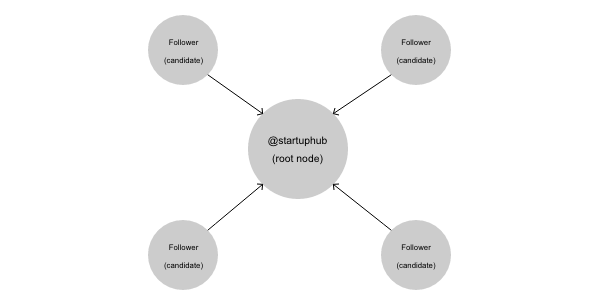
\includegraphics[width=1.0\textwidth]{root_node.png}
  \caption{The root node and Transnational Entrepreneur candidates.}
\end{figure}

\section{Root Network Extraction}
After identifying a Twitter User as your root node, the program will
extract a group of followers from your root node. These are your root
node's 1st degree network, or rather, an incomplete, directional,
egocentric network. This group of followers represent candidates for
Transnational Entrepreneurs, we use these users as candidates because
they are likely Entreprenuers in the city that we are interested in.
To determine whether they are the users that we are looking for, we
will perform a set of filters operations on them.

\section{Filter Level 0}
The first filter involved is named Filter level 0. Filter level 0 is
responsible for filtering the root node's followers to see whether
they are of interest. For the purposes of this research, we check two
things here.

\begin{itemize}
\item Is the User from Berlin?
\item Is the User a human?
\end{itemize}

The way we determine whether the User is from Berlin is by relying on
their time zone settings. We found that many users set their language,
or their city to whatever they would like, but the timezone, often
automatically set by the computer, is a good indicator of a user's
actual locale. Regardless, going with any one of the attributes is not
a completley valid way to ensure that a given user says where they
actually are, all information is subject to what the user wishes to
input.

The second criteria is a little bit more difficult to discern (is the
user human). It is not always possible to tell apart a human from a
robot or organization. In order to keep things as simple as possible,
we performed some basic checks that look for a valid ratio of
friends:followers, a limited amount of content repetition/spam, and
automatically passed them if they were Twitter verified. This is not a
foolproof way of filtering users as robots or not, but it is
computationally inexpensive and allowed us to move on to our next
stage of filtering. Further research could focus more on this aspect.

\section{Filter Level 1}
Filter level 1 is the part of the filtering process in which we
determine whether a user is of interest for further analysis. Exemple
gratia, are we going to gather their egocentric network? The reason
that we must assess this at this stage is because we are rate limited
in how many API calls we may make to the Twitter API for a given time
frame (please see the appendix for details). In order to assess
whether a candidate is therefore a transnational entrepreneur without
pulling their whole network, we pull a sample of their friends.

If we find that the sample distribution is valid, then we will mark
them as filtered and move on to processing them in the next stage. The
distribution ratio of a valid transnational is therefore that their
top two most common nationalaties in their network must be more than
\verb|50%| of their network and that their top two most common
nationalities may not differ by more than \verb|80%| in quantity.

\section{Transnational Entrepreneur Egocentric Network Extraction}
Following the selection of a set of individuals that we are interested
in, we begin the extraction process. We iterate through every
Transnational Entrepreneur candidate and collect a limited network of
their friends and followers. For our initial study, we limited this
network to a maximum of 200 friends and 200 followers for a given
Transnational Entrepreneur.

\section{Transnational Entrepreneur Egocentric Network Activity}
After extracting up to 200 friends and 200 followers from every given
Transnational Entreprenuer candidate, we gathered the latest 200
Tweets from every single user in the egocentric network. If the user
had Tweeted less than 200 total Tweets, we gathered all of their
Tweets.

\begin{figure}[H]
  \centering
  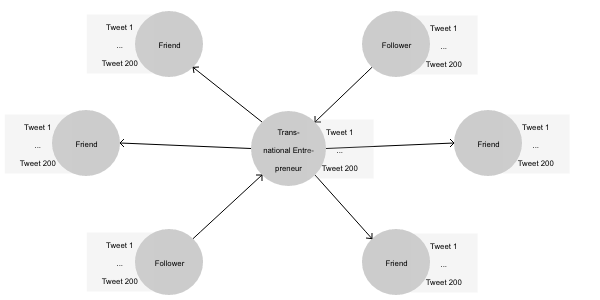
\includegraphics[width=1.0\textwidth]{tweets.png}
  \caption{A network graph of a Transnational Entrepreneur and thier Tweets.}
\end{figure}


By having a record of every single Tweet, and every single
timestamp from every Tweet, we can trace the diffusion of an idea
throughout a network. If we know that one of a Transantional
Entrepreneur's friends Tweeted about something, and then subsequently
the Transantional Entrepreneur Tweeted about the same topic, we can
assume with some degree of certainty that we witnessed information
diffusion from the friend of the Transnational Entrepreneur to the
Transnational Entrepreneur.

\section{Filter Level 2}
After collecting all of the Tweets from every single user of the
Transnational Entrepreneur's egocentric network, we now had the
capability to do more effective filtering for different indicators
that a given user may be a robot. In the case that a user is a robot,
we do not want to consider their data, our study is only concerned
with people. To quickly sort through hundreds of thousands of users we
take a number of shortcuts that are proxy indicators of humanity:

\begin{itemize}
\item Is the user Twitter verified?
\item Does the user have a valid ratio of friends to followers?
\item Does the user have enough statuses?
\item Is the user simply spamming the same Tweet over and over again?
\end{itemize}

\subsection{Is The User Twitter Verified}
One of the indicators we use to see whether a Twitter User's Tweets
are of human origin is whether they are verified or not. A verified
Twitter user is one that has submitted formal proof to Twitter that
they are who they say they are. Verified Twitter accounts are
therefore usually not spammers, and real people or organizations.

\subsection{User Friend to Follower Ratio}
A common technique by spam bots is to friend as many people as
possible in the hope that they will friend them back. They are
operating on the human reciprocity principle, and usually with rather
limited success. Because the amount of people that friend them back is
may be low, and far lower than it would be for most humans, we can
filter them out easily. We set a threshold of 10:1 friend to follower
ratio for someone to be considered human within our network. This
means that for every 10 people that they are friends with, they must
have at lest 1 follower, any less and they will be discounted.

\begin{figure}[H]
  \centering
  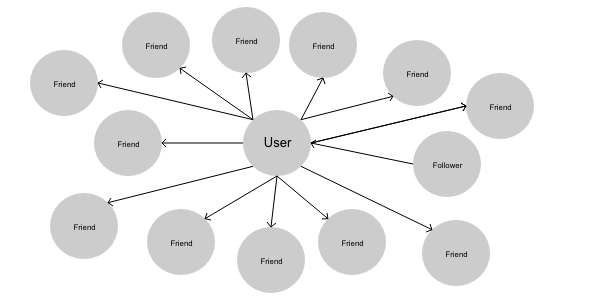
\includegraphics[width=1.0\textwidth]{friend_follower_ratio.png}
  \caption{An invalid friend to follower ratio.}
\end{figure}


\subsection{Minimum Status Requirements}
The minimum status requirements that we pose on a user are to make
sure that they are active on Twitter. We want to only pick up
individuals that are participating in conversations and contributing
to a community. For this reason we set a minimum number of statuses to
50, if a user has less than 50 statuses ever Tweeted, then they are
not considered in our computation.

\subsection{Is the User Spamming?}
Finally, the last thing that we can check, and the most
computationally expensive is- is the user spamming? To do this we
check the latest 200 of a user's total Tweets, if over \verb|50%| of
them are \verb|75%| or more similar, then we can conclude they are
likely spamming and we will not include their Tweets in our analysis.

\section{Diffusion Sequence Identification}
Following the collection of all of the Tweets within our network we
need to be able to identify diffusion of information. Because we have
a list of all the Tweets, and when they occured, we effectively have a
very large timeline of Tweets from the perspective of the
Transnational Entrepreneur. We canthen arrange them linearly and
replay the history of the network throughout time.

Throughout the replay of the network it is possible to look for the
following pattern from the perspective of the Transnational
Entrepreneur:

\begin{enumerate}
\item Country A - One of my friends posts a piece of information \verb|i| 
\item I pick up \verb|i| and post about it as well
\item Country B - One of my followers posts about \verb|i| after seeing my Tweet
\end{enumerate}

If this pattern can be observed, then an example of Transnational
Diffusion has been identified- a Tweet that somebody in one country
made, was transferred to another country via a Transnational
Entrepreneur. The Transnational Entrepreneur helped facilitate
information diffusion across borders.

Due to the high volume of Tweets within a network, doing this by hand
would be nearly impossible. In order to do this effectively, against
multiple Transnational Entrepreneur egocentric networks, machine
learning was utilized.

\section{Grouping Similar Tweets}
In order to group related Tweets together, there are a number of
possible clustering algorithms and document vectorization
schemes. Their needs and usefulness depends on the context, and nature
of the data, and the information known about that data, below, the
choices made for this research will be explained and justified.

\section{Document Tokenization \& Vectorization}
The first problem is: how to vectorize the documents (Tweets). To
vectorize documents means to create a simplified representation of a
document extracting all salient features for analysis (clusterization,
semantic analysis, etc). This simplified document representation
allows usage of a clustering or learning algorithm. It is important to
simplify and select only the most salient features of the document in
order to make the computation feasible. If you select the wrong
features or wrong parameters for your clustering, your model will be
effected by noise and contain false positives or false negatives.

For the purposes of this research, TF/IDF (term frequency/inverse
document frequency) was used in conjunction with a Porter
Stemmer. What this means is the following: If a word appears
frequently in a document, but infrequently in the other documents of a
collection, then, that word is more likely to be salient to the
context of that document.

To understand TF/IDF, consider a concrete example: A collection of
documents about legal issues. One of the documents is about the laws
in regards to birds. Naturally, within this special ``Bird Document''
one would expect significant usage of the world ``Bird'' or
``Aviary''. This word usage is compared to the frequency of ``Bird''
in other documents and is therefore marked as more important. The less
frequently ``Bird'' appears in other documents, the more related it is
to the ``Bird'' document. This helps filter out common words from the
whole document set that potentially carry less semantic meaning.

One issue that will immediately become apparent with a TF/IDF
vectorization is that synonyms would cause issues. If the ``Bird
Document'' uses several synonyms for birds, or mentions several
species of birds, the document may not record those words as salient
because individually they are not oft repeated, despite their
collective frequency within the whole document. For this reason,
a Porter Stemmer is used. A Porter Stemmer is a tool that can take
a given word and convert it to its ``base'' word. Consider the following
stem example:

\begin{enumerate}
\item Macaw
\item Parrot
\item Bird
\end{enumerate}

In the example, the word Macaw is simplified to Bird. Therefore, if
the document uses the word ``Parrot'' or ``Macaw'', both terms will be
classified as ``bird'' and the context of the document overall will be
more reliable, at the cost of less accuracy.

\section{DB Scan Clustering}
The clustering algorithm selected for this research was
DB-Scan. Initially K-Means was selected due to its fast performance
and the limited accesss to computational power, but it was deemed
unsuitable. The reason K-Means was deemed unsuitable, and the reason
DB-Scan was chosen is because DB-Scan does not require pre-defining
how many clusters exist in a given data set.

DB-Scan, roughly speaking, works by measuring the distance between two
vectors in a two dimensional space. If this distance is close enough,
these two vectors form the basis of a of a cluster. Iteratively
analayzing each vector reveals which vectors are all close enough to
each other to form a cluster. There are some settable parameters
within DB-Scan's implementation, particularly the Sci-kit Learn
implementation used in the research. For example, one can set what the
minimum threshold of related vectors to constitute a cluster. In
simpler terms, how many documents must be related for a cluster to be
considered a cluster. Additionally important is the ability to set the
threshold distance for two vectors to be related (known as
epsilon). This fine-tuning allows the data to be more accurately
grouped and categorized based on its nature.

Therefore, to breifly summarize, DB Scan was chosen because there were
an unknown quantity of content-clusters within the data set, and the
parameters available to tweak the behavior of the algorithm allowed
for fine grained adjustment of the similarity measure comparing two
vectors.
